\documentclass[conference]{IEEEtran}
\usepackage{cite}
\usepackage{amsmath,amssymb,amsfonts}
\usepackage{algorithmic}
\usepackage{graphicx}
\usepackage{textcomp}
\usepackage{xcolor}
\usepackage{hyperref}
\usepackage{tabularx}
\usepackage{lipsum}  
\usepackage{float}  

% COMMANDS
\newcommand{\R}{\mathbb{R}} \newcommand{\fig}[1]{\textit{Figure
\ref{#1}}} \newcommand{\eq}[1]{\textit{Equation \ref{#1}}}
\newcommand{\tabl}[1]{\textit{Table \ref{#1}}}
\newcommand{\addfigure}[3]{
    \begin{figure}
        \includegraphics[width=\linewidth]{#1}
        \caption{#2}
        \label{#3}
    \end{figure}
}
\begin{document}

% TITLE
\title{ - Applied AI in Biomedicine Workshop Report - Development of the HTF Deep-Learning Heartbeat Classifier   }

% AUTHORS
\author{ Alberto Rota \IEEEauthorblockA{ \\
    \textit{Person Code: 10615751}\\
    \textit{Student Number: 964662} \\
    \href{mailto:alberto2.rota@mail.polimi.it}{alberto2.rota@mail.polimi.it}}\\
\and
    Gabriele Santicchi \IEEEauthorblockA{ \\
    \textit{Person Code: 10579046}\\
    \textit{Student Number: 969088}  \\
    \href{mailto:gabriele.santicchi@mail.polimi.it}{gabriele.santicchi@mail.polimi.it}}
    }
\maketitle

\section{Context}
    The goal of this work is to build a classification model that
    properly annotates ECG heartbeats as Normal, PAC (supraventricular
    beats) or PVC (ventricular beats). The available dataset is
    composed of 2-lead ECG signal and R peaks position of 105 patient
    recordings. 

\section{Introduction}
    Electrocardiogram (ECG) signals record the electrical activity of
    the human heart and consist of several waveforms (P, QRS, and T).
    The duration and shape of each waveform and the distances between
    different peaks are used to diagnose Cardiovascular Heart Diseases
    (CVDs). Premature Atrial Contractions (PACs) and Premature
    Ventricular Contractions (PVCs) are among the most common forms of
    arrhythmias; the first results from premature electrical
    activation originating in the atria of the heart, while the second
    one is caused by a premature electrical activation originating in
    the ventricles. As the presence of frequent PACs and PVCs is
    associated with a higher risk of unfavorable prognosis
    \cite{relation_of} \cite{cardiac_mortality}, the accurate
    recognition of these abnormal beats is rigorously required. The
    aim of this work is to design a deep-learning ensemble model that
    properly classifies all the R-peaks in an ECG recording, without
    requiring the manual extraction of ECG features. The
    \textit{History-Time-Frequency} classifier analyzes each heartbeat
    in both the time and frequency domains, and take as input also the
    labels assigned to the previous two beats. 
    % The miss-classification error on the test set was around 3\%,
    % highlighting the potential of our classifier. 

    \addfigure
        {img/example.jpg} {Annotated ECGs from a sample patient}
        {fig:examples}

\subsection{Dataset}
    The dataset consists of 105 2-leads ECGs of 30 minutes recorded
    from 105 patients with two different sampling frequencies: more
    specifically, 65 patients were recorded with $f_s = 128 Hz$ and
    the remaining 40 patients with $f_s = 250Hz$. The recordings are
    annotated with the position of the R-peaks and their ground truth
    classification. An example is provided in \fig{fig:examples}.

\section{Data Preprocessing}
    The available raw dataset undergoes a pre-processing phase
    necessary for the optimal interfacing between the data and the
    model. 

\subsection{Exploratory Data Analysis}
    First and foremost, the acquisition frequencies are made uniform
    in the whole dataset by undersampling the recording acquired at
    $250Hz$: this is done in order to guarantee that the model inputs
    have the same size independently of the sampling frequency.  
    % This procedure is preferred to the oversampling of
    % low-resolution acquisition as it may introduce biases due to the
    % interpolation method. Moreover, the ECG features are preserved
    % after the undersampling, further justifying this choice. 

    No missing data is found in the recordings, hence there is no need
    to handle this kind of issue.
    

    An in-depth inspection of the dataset revealed, still, mismatches
    in the annotations of the R-peak positions, as for patient
    \textit{S005} and \textit{S009} the last heartbeat in the
    recording is labelled with a timestamp bigger than the signal
    length. In a conservative approach, given the very high number of
    heartbeats in the whole dataset (circa 244336), the two
    mislabelled R-peaks are removed.

    \addfigure
        {img/windowing.jpg} {Comparison of window splitting
        strategies. The \textit{RRR-based} (left) clearly shows
        inconsistency in the width; the \textit{fixed-width} (right)
        displays how adjacent peaks are included in the window; the
        \textit{adjusted RRR-based} (center) shows, in cases like the
        uppermost window, the padding used to match the dimensions}
        {fig:windowing}

    

\subsection{Signal Windowing}
    The heartbeat-by-heartbeat classification that the model performs
    implies the necessity of splitting the 30 minutes recording of
    each patient in windows, each one to be processed separately by
    the network: choosing the proper width and the optimal windowing
    approach is key in obtaining the best model performance. Three
    different approaches have been taken into consideration when
    splitting the windows:
    \begin{itemize}
        \item \textbf{RRR-based: }Each heartbeat is considered as
        starting from the R-peak of the previous one and ending to the
        R-peak of the following one (with some margin, 5\% of the
        window width by default, in order to not include the QR and RS
        slopes of the adjacent beats). This splitting strategy keeps
        the highest possible amount of information inside the window
        but, crucially, produces windows of inconsistent width, which
        depends on the patient heart-rate.
        \item \textbf{Fixed width: }A predefined width $w$ (in
        samples) is chosen and each window is considered as starting
        from $x_{peak}-w/2$ to $x_{peak}+w/2$. This approach assures a
        consistent window size and, additionally, makes sure that the
        R-peak is centered in the window. For patients with a high
        heart-rate though, adjacent R-peaks may be unavoidably
        included in the window.
        \item \textbf{Adjusted RRR-based: }This approach combines the
        two previously described strategies by initially performing
        the \textit{RRR-splitting} and later, after choosing a window
        width like in the \textit{fixed-width} approach, padding or
        cropping to the desired size. This approach makes sure that a
        single R-peak is contained in the window, and it assures a
        uniform width among all the splittings: to this extent, the
        informative content of the window is reduced by the least
        possible amount. 
    \end{itemize}

    \addfigure
        {img/histograms.jpg} {\textit{Left}: Distribution of the
        RR-interval in samples. \textit{Right}: Distribution of the
        distances between abnormal heartbeats. For example, most
        abnormal heartbeats (over 4500) are located 2 beats after the
        previous abnormal heartbeat } {fig:hists}

    \fig{fig:windowing} shows the effect of the above strategies. The
    \textit{adjusted RRR-based} is the employed windowing method, with
    the fixed width set at $w = 150$ samples, a value chosen based a
    qualitative analysis of the RR-interval distribution reported in
    \fig{fig:hists}. Once the ECG signals are split in windows, from
    the dataset tensor (of size $244336\times 150 \times 2$) 20\% of
    data is hold out to form the validation set and the remaining 10\%
    makes up the test set. The three datasets are standardized by the
    mean and standard deviation of the training set.     

\subsection{Class imbalance}
    As the following table highlights, the 244334 windows extracted
    (one for each available R-peak/heartbeat) are considerably
    unbalanced among the three labels of interest.
    \begin{center}
        \begin{tabular}{||c |c c c||}
            \hline
            & Normal & Sopraventricular & Ventricular \\
            \hline \hline
            Count & 226930 & 9609 & 7795 \\
            \hline
            Fraction & 92.87\% & 3.93\% & 3.19\% \\
            \hline
        \end{tabular}
    \end{center}

    
    \begin{figure*}
        \centering
        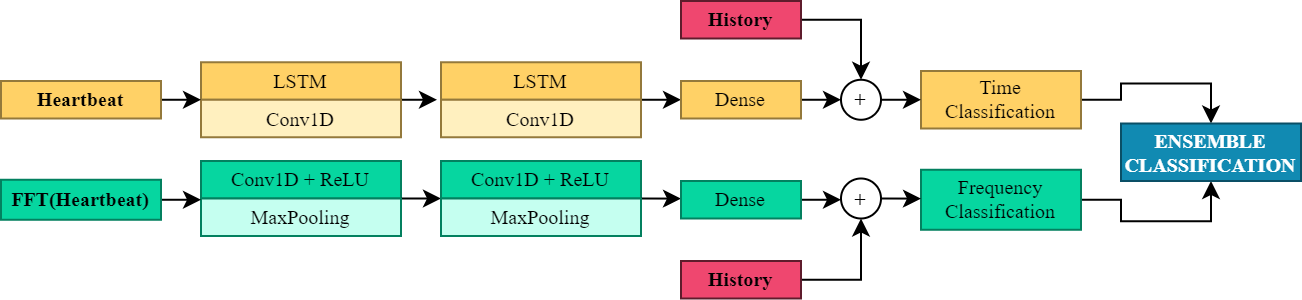
\includegraphics{img/model.png}
        \caption{Schematic of the History-Time-Frequency model
        ensemble, respectively color-coded in magenta, yellow and
        green}
        \label{fig:model}
    \end{figure*}

    If such an unbalanced dataset would be used to train the model,
    learning would occur only for the overrepresented class. As a
    consequence, the underrepresented pathological heartbeats would
    not be confidently classified: such model would have a very high
    specificity and a very low sensitivity. In order to cope with this
    kind of issue, an undersampling of the most frequent class has
    been performed to balance the class distribution. To do so,
    $\frac{7795}{105}$ Normal heartbeats have been randomly extracted
    from the ECG of each patient, obtaining a total of 7795 Normal
    peaks, a number equal to the least represented among the classes.

\section{The HTF Model}
    The proposed model is a \textit{History-Time-Frequency} ensemble
    (HTF), as the classification is performed in parallel in the Time
    domain and in the Frequency domain, while also accounting for
    History in terms of the labels of the past heartbeats in the ECG
    recording. 

\subsection{History}
    During a first inspection phase, an analysis on the distribution
    of pathological beats has been performed. In \fig{fig:hists}, the
    histogram reports the distribution of the abnormal interpeak
    distance computed over all the recordings, confirming that PACs
    and PVCs often occur in repeated patterns \cite{premature_v}
    \cite{frequent_premature} \cite{relation_of}. For these reasons, the involvement of
    the labels assigned to the previous peaks could help in predicting
    more precisely the label of the current peak. Considering the
    interpeak distance distributions, in this classifier the two
    previous labels have been added as additional inputs to the model.

\subsection{Time}
    One branch of the classifier consists of a recurrent architecture
    working on the ECG in time domain. Here, Long Short-Term Memories
    (LSTMs) in combination with 1D convolutions are employed to
    extract the most relevant features of the ECG morphology while
    accounting for their temporal dependencies. The heartbeat history
    is concatenated to the network prior to the last Dense+Softmax
    layer, so that the final labelling decision also accounts for the
    past two labels: the concatenation operation prior to the final
    classifier layer allows the model to learn how to combine the
    information about the current peak with the information related to
    the history.

\subsection{Frequency}
    The last branch of this model consists in a frequency-domain
    classifier on a Fourier Transform of the inputs. In order to apply
    the Fourier Transform, the \textit{quasi}-stationarity hypothesis
    has been assumed for each window.
    %  This is not an heavy assumption, since the inputs length is
    % very short and most part of the window consists in the peak
    % recorded. 
    The classifier consist of multiple CNN-ReLU-MaxPooling stacks. A
    small convolutional kernel has been chosen to extract features at
    a reduced scale. After the application of the FFT on the input
    signal, the output of the CNN layer is concatenated with the two
    history labels like in the time model. Finally, a dense layer with
    a softmax activation function provides the probability assigned to
    the three classes.  

    The full ensemble model is schematically represented in
    \fig{fig:model}.

\section{Training}
    The time and frequency models have been trained separately and
    then ensembled by summing the class probability vectors. The
    training is performed by minimizing a Categorical Crossentropy
    loss function with the ADAM optimizer. The training phase of the
    time model is set up for 100 epochs, while the frequency model
    fits over thrice the epochs as it has been observed converging at
    a slower rate. Batch size is of 256 heartbeats, learning rate
    starts from $1\cdot10^{-3}$ and decreases on eventual loss
    plateaus. Training is monitored on accuracy and on a recall metric
    calculated per class, as follows:
    \begin{equation}
        Recall_k=\frac{True_k}{True_k+\sum_{i=0}^{classes}False_i}
    \end{equation}
    This metric allows to evaluate if the class imbalance issue has
    been correctly resolved, as an imbalanced dataset will reflect on
    a low recall for the underrepresented classes. Training histories
    are reported on \fig{app:training}.

\section{Results}
    Results have been evaluated in terms of the model precision,
    recall and f1-score on the 3 classes separately. The test set used
    for such evaluation consists of 10\% of the available dataset.
    
    \begin{center}
        \begin{tabular}{||c|c c c c||}
            \hline
            Label & Precision & Recall & f1-score & Support\\
            \hline \hline
        
            Normal& 0.98&0.96&0.97&699\\
            \hline
            Sopraventricular& 0.96&0.98&0.97&865\\
            \hline
            Ventricular& 0.98&0.98&0.98&702\\
            \hline\hline
        
            Per-Class Accuracy &0.97&0.97&0.97&2266\\
            \hline
            Weighted Accuracy &0.97&0.97&0.97&2266\\
            \hline
            Overall Accuracy&&&&\textbf{0.97}\\
            \hline
        \end{tabular}
    \end{center}

    The same results are graphically represented in the form of a
    confusion matrix in \fig{fig:confmat}, this time differentiating
    the results of the time model, the frequency model and the
    ensemble.

    \begin{figure*}
        \centering
        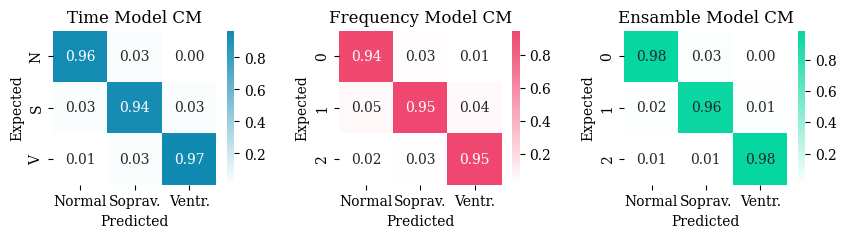
\includegraphics[width=\linewidth]{img/confmatr.png}
        \caption{}
        \label{fig:confmat}
    \end{figure*}

\section{Discussion}
    Results from the test set show that the HTF model performs equally good on
    the three classes: this is due to the balancing phase performed before
    training. Moreover, the undersampling strategy used in the balancing
    stage led to a reduced training time with no evidence of overfitting.

    The window splitting method represents a fundamental part of the entire
    work; the \textbf{Adjusted RRR-based} has been chosen to train the HTF model for mainly two reasons.
    First, it assures the window to have a fixed length, with a single peak in
    the middle; this improves the performance of the model because it intrinsically learns that the 
    most important features are located in the middle of the array/input.
    The padding that has been performed was necessary since it is necessary to
    avoid the presence of multiple peaks in a single window, which is generally
    caused by arrythmias or tachicardic conditions. Among  all the 
    splitting method tested, this one got the best results and so it has been 
    chosen for the deployment of the final model. 

    As PACs and PVCs often occurs in a repetitive fashion \cite{premature_v}, a number of past
    labels has been included as model inputs to consider also the history 
    of the signal. Even if a great number of
    past classifications could lead to better overall performances, no
    significant improvement has been observed both on time and frequency 
    models when including more than two labels.
    % so this latter
    % has been chosen for the final development.
    
    Both the time and frequency model got high performances on all the three 
    classes. Moreover, they performed better on different classes: the time 
    model classifies well the <normal and PVC>s, 
    while the frequency one the PACs class. These results led to development 
    of an ensemble model which combine the output probabilities of the two, 
    in order to strenghten the classifier accuracy. 

\section{Conclusions}
    In this work a History-Time-Frequency model has been developed in order 
    to classify the heart peaks in ECG signal of a patient as normal,
    Sopraventricular or Ventricular. 
    The model performance has been assessed by the means of different metrics, 
    such as accuracy, sensitivity and specificity; results on the test set 
    highlight the <strength> of this ensemble classifier, which got a 97\%
    accuracy on average.

% BIBLIOGRAPHY
\bibliography{biblio.bib}
\bibliographystyle{plain}
\newpage
% APPENDIX
\appendices
\begin{figure*}
    \centering
    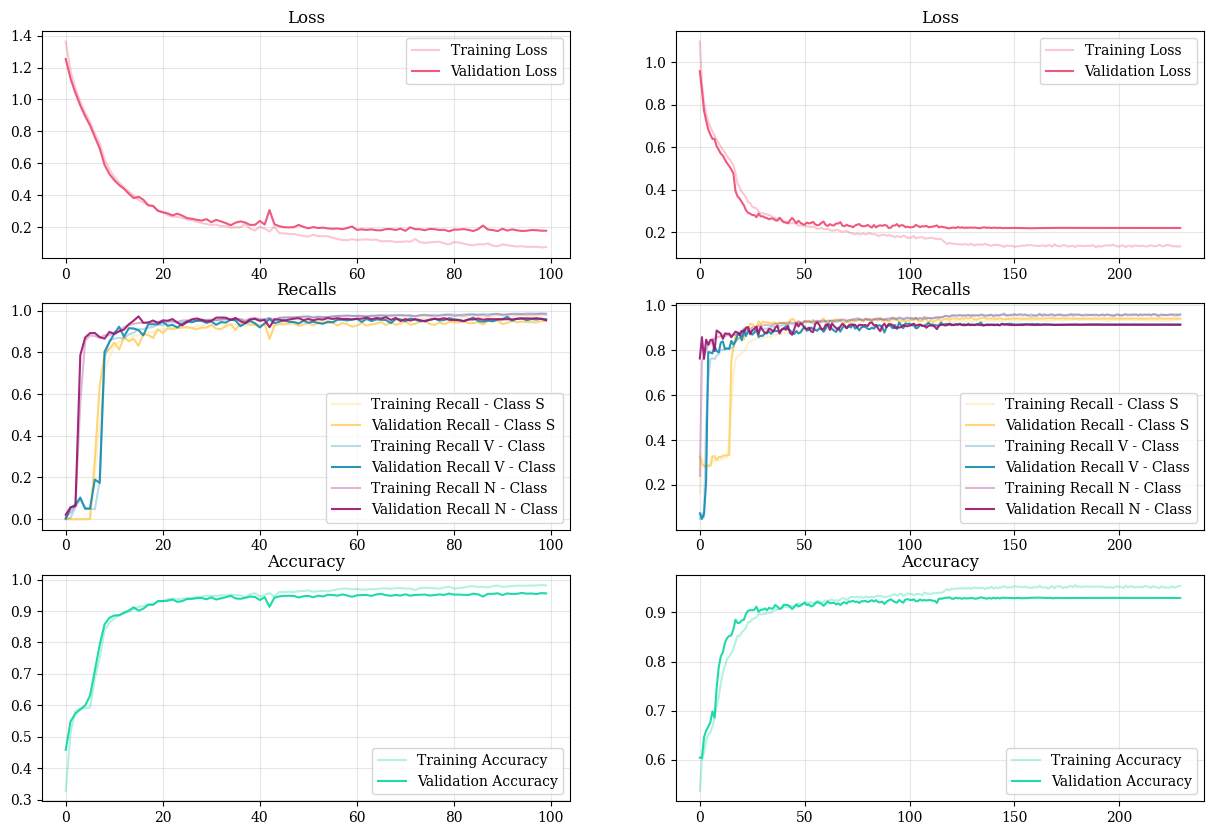
\includegraphics[width=\linewidth]{img/training.png}
    \caption{}
    \label{app:training}
\end{figure*}
\section{Training Process}


\end{document}